\documentclass[a4j,papersize]{jsbook}

\usepackage[T1]{fontenc} % LaTeXのフォントのエンコーディングをT1にする
\usepackage{textcomp} % TS1
\usepackage[utf8]{inputenc} % ファイルのエンコーディングをUTF8にする
\usepackage{lmodern}

\usepackage{url}

\usepackage{document} % 自作書式集

%%%%%%%%%%%%%%%%%%%%%%%%%%%%%%%%%%%%%%%%%%%%%%%%%%%%%%%%%%%%%%%%%%%%%%%%%%%%%%
% 本文
%%%%%%%%%%%%%%%%%%%%%%%%%%%%%%%%%%%%%%%%%%%%%%%%%%%%%%%%%%%%%%%%%%%%%%%%%%%%%%

%\title{オブジェクト指向フレームワーク原論}
\title{Javaによる抽象化プログラミング技法}
\author{中鉢 欣秀}
\begin{document}
\maketitle
% \tableofcontents

\chapter*{序}

\begin{abstract}
寿限無寿限無五劫の摺り切れ海砂利水魚の水行末雲来末風来末.食う寝る所に住む所藪柑子ブラコウジ.パイポパイポパイポのシューリンガングーリンダイのポンポコピーのポンポコナーの長久命の長助.
\end{abstract}

\section*{はじめに}

この教科書はオブジェクト指向の初心者が最短でオブジェクト指向の抽象化機
構を最短で理解できることを目指します.

ソフトウェアに関連する技術の移り変わりはとても早い.変わらない知識(普遍的な知識)を身につけることこそ,ソフトウェアのアーキテクトに求められることです.

ソフトウェア・アーキテクチャに関する本質的な知識.

オブジェクト指向の概念に基づくCBD(Component Based Development)を主要なトピックとします.
フレームワークの作り方を学ぶことで,上手な使い方を体得することが目標です.

フレームワークを作れるようになろう 

他人の作ったフレームワークを使って満足するだけ
でよいのか? 

フレームワークを使えるようになろう 

フレームワークの作り方を学ぶことによって、既存
フレームワークをより深く理解することができる 

フレームワーク・プログラミングをとりあげる
理由 

ソフトウェア開発においては、ソフトウェアを部品
化(コンポーネント化)し、部品を再利用すること
で開発効率を上げるための試みが行われてきた。 

フレームワークの構築 

原始的なIPO構造の理解から順をおって、フレーム
ワーク構築までを行ないます。 

オブジェクト指向の最も有用な利用方法の一つとし
てフレームワークとプラグインによるアーキテク
チャ設計を理解しましょう。 

汎用的な技術 

ソフトウェアにおける「構造」とは? 

オブジェクト指向によるフレームワークの設計 

応用的な技術 

Eclipseとプラグインを活用したソフトウェア開発 

実践的なフレームワークのアーキテクチャ 

ソフトウェアの中核的構造をフレームワークとして設計す
る考え方が普及した。 

目的に応じたコンポーネントをフレームワークにプ
ラグインすることで、最も重要で複雑な中核部分の
構造を再利用できるようにする。 

こうすることにより、プログラミングにおける省力化が達
成される。


javaの約束事や決まりごとは「おまじない」または「お約束」と説明するのが
慣例です.
このテキストでは,明確にそれらの解説への参照箇所を示します.

Java言語は初心者向けの言語ではありません.ごく簡単なプログラムであって
もいわゆる「おまじない」がいっぱい出てきます.

Java仕様書

\url{http://docs.oracle.com/javase/specs/jls/se7/jls7-diffs.pdf}

IPOフレームワーク

MVCフレームワーク

\chapter{フレームワークとはなにか}

\begin{abstract}
寿限無寿限無五劫の摺り切れ海砂利水魚の水行末雲来末風来末.食う寝る所に住む所藪柑子ブラコウジ.パイポパイポパイポのシューリンガングーリンダイのポンポコピーのポンポコナーの長久命の長助.
\end{abstract}

\section{フレームワークの定義}
フレームワークの一般的な定義 

1.抽象クラスの集合とそのインスタンス間の相互
作用によって表現された,システムの全体または一
部の再利用可能な設計 

2.開発者がカスタマイズできる,アプリケーショ
ンの骨組み 

 出典) R.ジョンソン,中村宏明,中山裕子,吉田和樹著,
「パターンとフレームワーク」,共立出版 

\section{フレームワークの重要な性質}
ハリウッド・プリンシプル 

映画監督のセリフ 

「Don’t call me, I call you」 

 ハリウッドの役者は,仕事が来るのをひたすら家で待って
いなくてはならない,という例え 

フレームワークは映画監督 

フレームワークの利用者が作成するコンポーネント
は,フレームワークを呼び出すのではなく,フレー
ムワークに呼び出されるのを待つ 

% スライドp19まで

%trim option's parameter order: left bottom right top
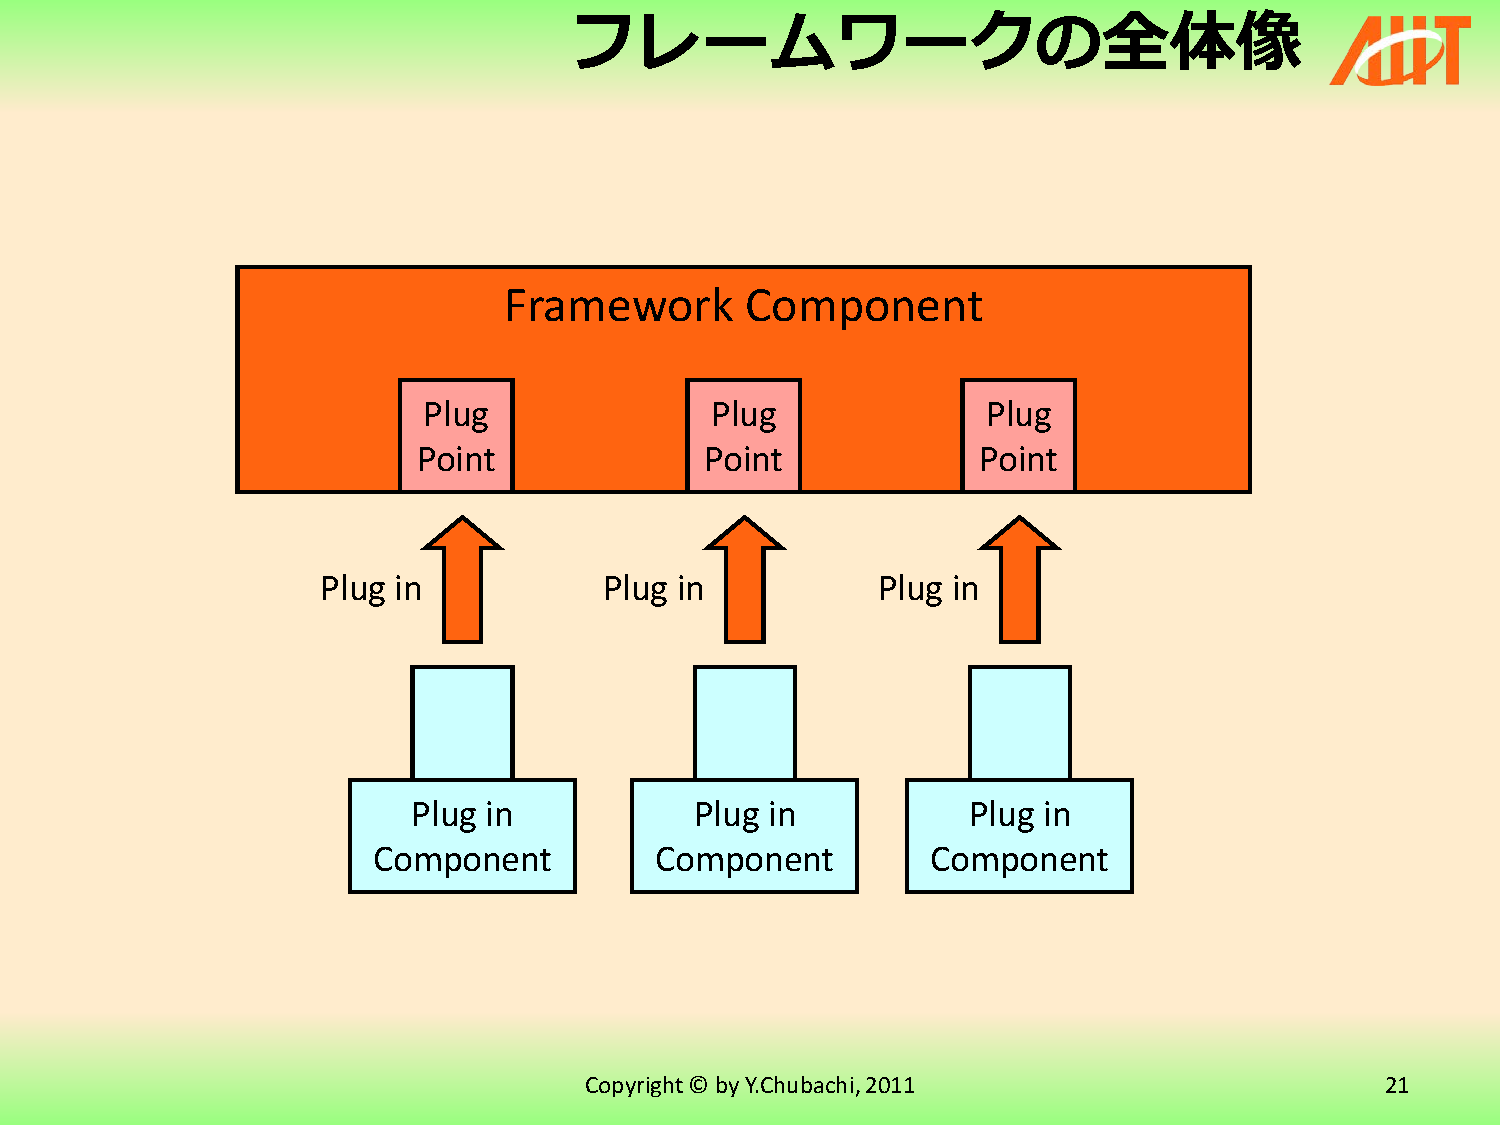
\includegraphics[width=0.8\textwidth, trim=30mm 30mm 35mm 35mm,clip]{framework.pdf}


\chapter{プログラムのアーキテクチャ}

\begin{abstract}
寿限無寿限無五劫の摺り切れ海砂利水魚の水行末雲来末風来末.食う寝る所に住む所藪柑子ブラコウジ.パイポパイポパイポのシューリンガングーリンダイのポンポコピーのポンポコナーの長久命の長助.
\end{abstract}

\section{自乗を計算するプログラム}
\begin{figure}
\begin{Verbatim}[commandchars=\\\{\},numbers=left,firstnumber=1,stepnumber=1,frame=single,fontsize=\small]
\PY{k+kn}{package}\PY{+w}{ }\PY{n}{square}\PY{o}{;}

\PY{k+kn}{import}\PY{+w}{ }\PY{n+nn}{java.io.BufferedReader}\PY{o}{;}
\PY{k+kn}{import}\PY{+w}{ }\PY{n+nn}{java.io.InputStreamReader}\PY{o}{;}

\PY{k+kd}{public}\PY{+w}{ }\PY{k+kd}{class}\PY{+w}{ }\PY{n+nc}{Square}\PY{+w}{ }\PY{o}{\PYZob{}}
\PY{+w}{    }\PY{k+kd}{public}\PY{+w}{ }\PY{k+kd}{static}\PY{+w}{ }\PY{k+kt}{void}\PY{+w}{ }\PY{n+nf}{main}\PY{o}{(}\PY{n}{String}\PY{o}{[}\PY{o}{]}\PY{+w}{ }\PY{n}{args}\PY{o}{)}\PY{+w}{ }\PY{k+kd}{throws}\PY{+w}{ }\PY{n}{Exception}\PY{+w}{ }\PY{o}{\PYZob{}}
\PY{+w}{    }\PY{+w}{    }\PY{n}{Square}\PY{+w}{ }\PY{n}{square}\PY{+w}{ }\PY{o}{=}\PY{+w}{ }\PY{k}{new}\PY{+w}{ }\PY{n}{Square}\PY{o}{(}\PY{o}{)}\PY{o}{;}
\PY{+w}{    }\PY{+w}{    }\PY{n}{square}\PY{o}{.}\PY{n+na}{run}\PY{o}{(}\PY{o}{)}\PY{o}{;}
\PY{+w}{    }\PY{o}{\PYZcb{}}

\PY{+w}{    }\PY{k+kd}{private}\PY{+w}{ }\PY{k+kt}{void}\PY{+w}{ }\PY{n+nf}{run}\PY{o}{(}\PY{o}{)}\PY{+w}{ }\PY{k+kd}{throws}\PY{+w}{ }\PY{n}{Exception}\PY{+w}{ }\PY{o}{\PYZob{}}
\PY{+w}{    }\PY{+w}{    }\PY{n}{System}\PY{o}{.}\PY{n+na}{out}\PY{o}{.}\PY{n+na}{print}\PY{o}{(}\PY{l+s}{"自乗を計算する値を入力してください:"}\PY{o}{)}\PY{o}{;}
\PY{+w}{    }\PY{+w}{    }\PY{n}{BufferedReader}\PY{+w}{ }\PY{n}{reader}\PY{+w}{ }\PY{o}{=}
\PY{+w}{    }\PY{+w}{    }\PY{+w}{    }\PY{k}{new}\PY{+w}{ }\PY{n+nf}{BufferedReader}\PY{o}{(}
\PY{+w}{    }\PY{+w}{    }\PY{+w}{    }\PY{+w}{    }\PY{k}{new}\PY{+w}{ }\PY{n+nf}{InputStreamReader}\PY{o}{(}\PY{n}{System}\PY{o}{.}\PY{n+na}{in}\PY{o}{)}\PY{o}{)}\PY{o}{;}
\PY{+w}{    }\PY{+w}{    }\PY{n}{String}\PY{+w}{ }\PY{n}{valueString}\PY{+w}{ }\PY{o}{=}\PY{+w}{ }\PY{n}{reader}\PY{o}{.}\PY{n+na}{readLine}\PY{o}{(}\PY{o}{)}\PY{o}{;}
\PY{+w}{    }\PY{+w}{    }\PY{k+kt}{double}\PY{+w}{ }\PY{n}{value}\PY{+w}{ }\PY{o}{=}\PY{+w}{ }\PY{n}{Double}\PY{o}{.}\PY{n+na}{parseDouble}\PY{o}{(}\PY{n}{valueString}\PY{o}{)}\PY{o}{;}
\PY{+w}{    }\PY{+w}{    }\PY{n}{System}\PY{o}{.}\PY{n+na}{out}\PY{o}{.}\PY{n+na}{println}\PY{o}{(}\PY{l+s}{"計算結果:"}\PY{+w}{ }\PY{o}{+}\PY{+w}{ }\PY{o}{(}\PY{n}{value}\PY{+w}{ }\PY{o}{*}\PY{+w}{ }\PY{n}{value}\PY{o}{)}\PY{o}{)}\PY{o}{;}
\PY{+w}{    }\PY{o}{\PYZcb{}}
\PY{o}{\PYZcb{}}
\end{Verbatim}

\caption{自乗を計算するプログラム}\label{code:Square1:square:Square}
\end{figure}

図\ref{code:Square1:square:Square}は,Squareという名前のクラスを定義する
コードです.

1行目はパッケージ宣言です(正式は?)\marginpar{パッケージについて
は・・・を参照.}.

それでは,次の例題を考えてみましょう.

\begin{例題}
 図\ref{code:Square1:square:Square}の\texttt{run()}メソッド内のコー
 ドを入力・処理・出力のパターンで分類せよ.
\end{例題}

寿限無寿限無五劫の摺り切れ海砂利水魚の水行末雲来末風来末.食う寝る所に住む所藪柑子ブラコウジ.パイポパイポパイポのシューリンガングーリンダイのポンポコピーのポンポコナーの長久命の長助
\marginpar{寿限無寿限無五劫の摺り切れ海砂利水魚の水行末雲来末風来末.食う寝る所に住む所藪柑子ブラコウジ.パイポパイポパイポのシューリンガングーリンダイのポンポコピーのポンポコナーの長久命の長助.}
.

\section{演習問題}

\begin{演習}
 Java言語ではクラスの名前とファイル名を一致させる必要がある.他のオブジェ
 クト指向型言語の場合を調べよ.また,クラス名とファイル名を一致させるこ
 との長所・短所について考察せよ.
\end{演習}

\begin{演習}
 図\ref{code:Square1:square:Square}の・・・を・・・せよ.
\end{演習}

\begin{演習}
 図?は割り算をして商とあまりを計算するプログラムです.
 コメントブロックを用いて,このプログラムを入力・処理・出力に整理しなさい
 \end{演習}
 
\begin{figure}
\begin{Verbatim}[commandchars=\\\{\},numbers=left,firstnumber=1,stepnumber=1,frame=single,fontsize=\small]
\PY{k+kn}{import}\PY{+w}{ }\PY{n+nn}{java.io.BufferedReader}\PY{o}{;}
\PY{k+kn}{import}\PY{+w}{ }\PY{n+nn}{java.io.InputStreamReader}\PY{o}{;}


\PY{k+kd}{public}\PY{+w}{ }\PY{k+kd}{class}\PY{+w}{ }\PY{n+nc}{Division}\PY{+w}{ }\PY{o}{\PYZob{}}
\PY{+w}{    }\PY{k+kd}{public}\PY{+w}{ }\PY{k+kd}{static}\PY{+w}{ }\PY{k+kt}{void}\PY{+w}{ }\PY{n+nf}{main}\PY{o}{(}\PY{n}{String}\PY{o}{[}\PY{o}{]}\PY{+w}{ }\PY{n}{args}\PY{o}{)}\PY{+w}{ }\PY{k+kd}{throws}\PY{+w}{ }\PY{n}{Exception}\PY{+w}{ }\PY{o}{\PYZob{}}
\PY{+w}{    }\PY{+w}{    }\PY{n}{Division}\PY{+w}{ }\PY{n}{division}\PY{+w}{ }\PY{o}{=}\PY{+w}{ }\PY{k}{new}\PY{+w}{ }\PY{n}{Division}\PY{o}{(}\PY{o}{)}\PY{o}{;}
\PY{+w}{    }\PY{+w}{    }\PY{n}{division}\PY{o}{.}\PY{n+na}{run}\PY{o}{(}\PY{o}{)}\PY{o}{;}
\PY{+w}{    }\PY{o}{\PYZcb{}}
\PY{+w}{    }
\PY{+w}{    }
\PY{+w}{    }\PY{k+kd}{private}\PY{+w}{ }\PY{k+kt}{void}\PY{+w}{ }\PY{n+nf}{run}\PY{o}{(}\PY{o}{)}\PY{+w}{ }\PY{k+kd}{throws}\PY{+w}{ }\PY{n}{Exception}\PY{+w}{ }\PY{o}{\PYZob{}}
\PY{+w}{    }\PY{+w}{    }\PY{c+c1}{//}\PY{+w}{ }\PY{c+c1}{割られる数と割る数を読み込む}
\PY{+w}{    }\PY{+w}{    }\PY{n}{BufferedReader}\PY{+w}{ }\PY{n}{reader}\PY{+w}{ }\PY{o}{=}
\PY{+w}{    }\PY{+w}{    }\PY{+w}{    }\PY{k}{new}\PY{+w}{ }\PY{n+nf}{BufferedReader}\PY{o}{(}\PY{k}{new}\PY{+w}{ }\PY{n}{InputStreamReader}\PY{o}{(}\PY{n}{System}\PY{o}{.}\PY{n+na}{in}\PY{o}{)}\PY{o}{)}\PY{o}{;}
\PY{+w}{    }\PY{+w}{    }\PY{n}{System}\PY{o}{.}\PY{n+na}{out}\PY{o}{.}\PY{n+na}{print}\PY{o}{(}\PY{l+s}{"割られる数を入力してください:"}\PY{o}{)}\PY{o}{;}
\PY{+w}{    }\PY{+w}{    }\PY{n}{String}\PY{+w}{ }\PY{n}{dividendString}\PY{+w}{ }\PY{o}{=}\PY{+w}{ }\PY{n}{reader}\PY{o}{.}\PY{n+na}{readLine}\PY{o}{(}\PY{o}{)}\PY{o}{;}
\PY{+w}{    }\PY{+w}{    }\PY{k+kt}{int}\PY{+w}{ }\PY{n}{dividend}\PY{+w}{ }\PY{o}{=}\PY{+w}{ }\PY{n}{Integer}\PY{o}{.}\PY{n+na}{parseInt}\PY{o}{(}\PY{n}{dividendString}\PY{o}{)}\PY{o}{;}
\PY{+w}{    }\PY{+w}{    }\PY{n}{System}\PY{o}{.}\PY{n+na}{out}\PY{o}{.}\PY{n+na}{print}\PY{o}{(}\PY{l+s}{"割る数を入力してください:"}\PY{o}{)}\PY{o}{;}
\PY{+w}{    }\PY{+w}{    }\PY{n}{String}\PY{+w}{ }\PY{n}{divisorString}\PY{+w}{ }\PY{o}{=}\PY{+w}{ }\PY{n}{reader}\PY{o}{.}\PY{n+na}{readLine}\PY{o}{(}\PY{o}{)}\PY{o}{;}
\PY{+w}{    }\PY{+w}{    }\PY{k+kt}{int}\PY{+w}{ }\PY{n}{divisor}\PY{+w}{ }\PY{o}{=}\PY{+w}{ }\PY{n}{Integer}\PY{o}{.}\PY{n+na}{parseInt}\PY{o}{(}\PY{n}{divisorString}\PY{o}{)}\PY{o}{;}
\PY{+w}{    }\PY{+w}{    }
\PY{+w}{    }\PY{+w}{    }\PY{c+c1}{//}\PY{+w}{ }\PY{c+c1}{商と余を計算する}
\PY{+w}{    }\PY{+w}{    }\PY{k+kt}{int}\PY{+w}{ }\PY{n}{quotient}\PY{+w}{ }\PY{o}{=}\PY{+w}{ }\PY{n}{dividend}\PY{+w}{ }\PY{o}{/}\PY{+w}{ }\PY{n}{divisor}\PY{o}{;}
\PY{+w}{    }\PY{+w}{    }\PY{k+kt}{int}\PY{+w}{ }\PY{n}{remainder}\PY{+w}{ }\PY{o}{=}\PY{+w}{ }\PY{n}{dividend}\PY{+w}{ }\PY{o}{\PYZpc{}}\PY{+w}{ }\PY{n}{divisor}\PY{o}{;}

\PY{+w}{    }\PY{+w}{    }\PY{c+c1}{//}\PY{+w}{ }\PY{c+c1}{割り算の結果を表示する}
\PY{+w}{    }\PY{+w}{    }\PY{n}{System}\PY{o}{.}\PY{n+na}{out}\PY{o}{.}\PY{n+na}{print}\PY{o}{(}\PY{l+s}{"商は"}\PY{+w}{ }\PY{o}{+}\PY{+w}{ }\PY{n}{quotient}\PY{+w}{ }\PY{o}{+}\PY{+w}{ }\PY{l+s}{"で余は"}\PY{+w}{ }\PY{o}{+}\PY{+w}{ }\PY{n}{remainder}\PY{+w}{ }\PY{o}{+}\PY{+w}{ }\PY{l+s}{"です"}\PY{o}{)}\PY{o}{;}
\PY{+w}{    }\PY{o}{\PYZcb{}}

\PY{o}{\PYZcb{}}
\end{Verbatim}

\caption{割り算をするプログラム} 
\end{figure}

\section{パッケージとクラスの可視性}
パッケージは名前空間です.

\chapter{メモ}

\begin{enumerate}
 \item 名前付けと抽象化について(int x = 1; double pi = 3.14)
 \item テストを取り上げるか?
 \item パターンとアーキテクチャについて解説する?
\end{enumerate}

\end{document}
